\section{Introduction}
\label{sec:intro}

This report use sketching methods to deal with the
least square problem which minimizes
\begin{equation} \label{eq:ls}
    f(x) = \frac{1}{\sqrt{n}} \|Ax-b\|_2,
\end{equation}
where $A\in\real^{n\times d}$, $b\in\real^n$, and $x\in\real^d$.
We use the \emph{how much did it rain ii} \cite{rain, Lakshmanan16}
dataset from \emph{kaggle.com} for the analysis of different sketching methods.
The original dataset contains 13,765,201 training samples
with 23 features and 1 prediction value.
See the Appendix for detailed description of features.
Since it contains null values and outliers,
we will do a preprocess and only use a subset of samples.

\subsection{Preprocess and Baselines}

Since some observations are not complete,
we first filter out 2,769,088 samples that do not contain missing values.
The first two features \emph{id} and \emph{minutes\_past}
are used just for identification rows,
thus we omit them and
get data matrices
\begin{equation}
    A_0 \in \real^{2769088\times 21}, \,
    b_0\in\real^{2769088}.
\end{equation}
The distribution of these inputs was shown in Figure~\ref{fig:box}.
\begin{figure}[htb]
	\centering
	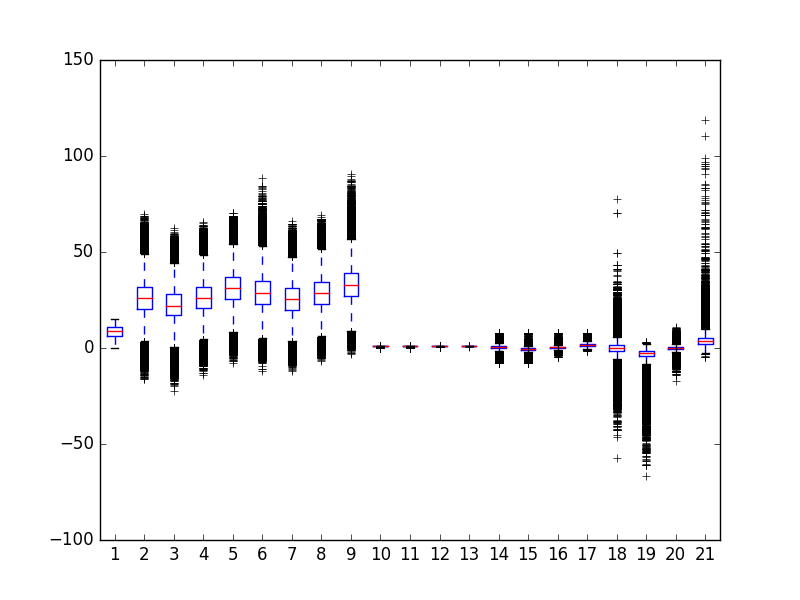
\includegraphics[height=6cm]{fig/box_a_0.png}
	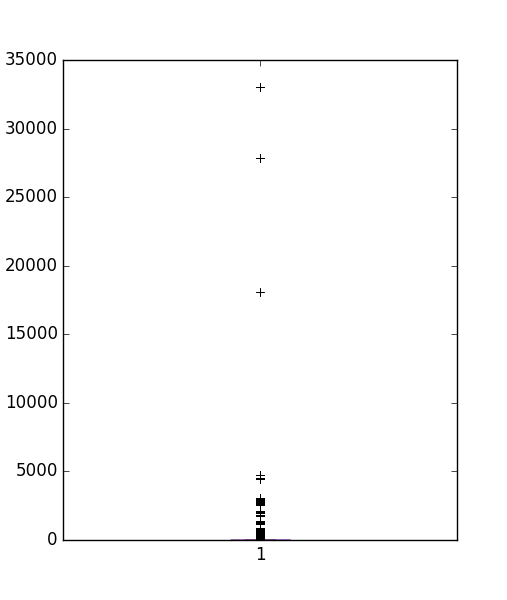
\includegraphics[height=6cm]{fig/box_b_0.png}
	\caption{\small
		Left, box plot for columns of $A_0$.
        Right, that for $b_0$.
        We can see $b_0$ contains outliers.}
	\label{fig:box}
\end{figure}

Firstly, direct compute the least square problem \eqref{eq:ls}
by equation
\begin{equation} \label{eq:psudo}
    x_0^*=(A_0^TA_0)^{-1}A_0^Tb_0.
\end{equation}
we get
$$
    x_0^*=(0.758, 0.046, 0.218, \dots, -0.035, -0.101)
$$
with loss $f(x_0^*) = 156.1$ in $0.24$ seconds.
Compared to $12.2$, the mean value of $b_0$,
the loss seems too large.
The $99$-th percentile of prediction values in $b_0$ is $144$.
We then use samples that have prediction values less than $144$
and get new data
\begin{equation}
    A \in \real^{2741220\times 21}, \,
    b\in\real^{2741220}.
\end{equation}
Directly compute using Equation~\eqref{eq:psudo} again, we have
$$
    x^*=(0.189, -0.012, -0.008, \dots, 0.042, -0.040)
$$
with loss $f(x^*) = 9.11$ in $0.24$ seconds.
This makes more sense because
$\text{mean}(b)=4.24$,
$\text{std}(b) = 9.30$,
$\text{minimum}(b) = 0.01$, and
$\text{maximum}(b) = 142.2$.
And this serves as the baseline for our later discussion.
